\chapter{基于友邻训练的对话语义理解}
\label{cha:fdt}
本章专注于提升聊天机器人理解对话语义的能力。对话语义角色标注和对话重写是两个让模型理解对话语义的任务,但是这两个任务目前缺乏高质量的训练数据。本章将自训练和多任务结合,提出了一个新的半监督学习框架来利用大规模无标注数据生成高质量的伪标签,用于训练模型。具体而言,\ref{sec:fdt-intro}节用具体的例子阐释了新框架的主要思想并引出全文;\ref{sec:fdt_framework}节详细介绍了新框架的原理;\ref{sec:fdt_model}节介绍了如何在对话语义角色标注和对话重写两个任务上使用新框架;\ref{sec:fdt_exp}节利用实验证明了新框架的有效性;最后\ref{sec:fdt_conclusion}节总结本章内容。

\section{引言}\label{sec:fdt-intro}

许多不同的机器学习算法,例如⾃监督学习~\cite{Mikolov2013-mr,devlin2018bert,liu2021self},半监督学习~\citep{yang2021survey}和弱监督
学习~\cite{zhou2018brief},旨在使⽤无标注的数据来提⾼模型性能。由于目前互联网上有大量可⽤的无标注数据,这些方法最近引起了研究者很大的兴趣。⾃训练~\cite{scudder1965probability}是⼀种半监督学习方法,旨在通过伪标签来提升模型性能,并已成功应用于计算机视觉~\cite{lee2013pseudo,chen2021semi},自然语言处理 ~\cite{dong2011ensemble,bhat2021self},和其他领域~\cite{wang2019attributed,kahn2020self}。

自训练的主要挑战是如何选择高质量的伪标签。当前的⾃训练算法在评估伪标签的质量时主要关注单个任务并会因为受到噪声数据的影响~\cite{zhang2021understanding}。本章⼯作的动机是不同任务的学习⽬标代表输⼊的不同属性,并且⼀些属性在任务之间共享,可以⽤作从⼀个任务到另⼀个任务的监督信号。这些属性包括依存句法分析和成分句法分析中的某些跨度边界,以及情感分析和情绪识别中的某些情感极性。两个对话理解任务,对话语义角色标注(Conversational Semantic Role Labeling, CSRL)和对话重写(Dialogue Rewriting, DR)也是这样的⼀对任务,它们具有共指和零代词解析等共享属性。如图\ref{fig:fdt_intro}所示,重写的话语产生对于谓词“喜欢”的参数的跨任务监督信号。本章利用来自友邻任务(不同但相关的任务)之间的跨任务监督信号作为评估伪标签质量的重要标准。

\begin{figure}[!t]
\centering
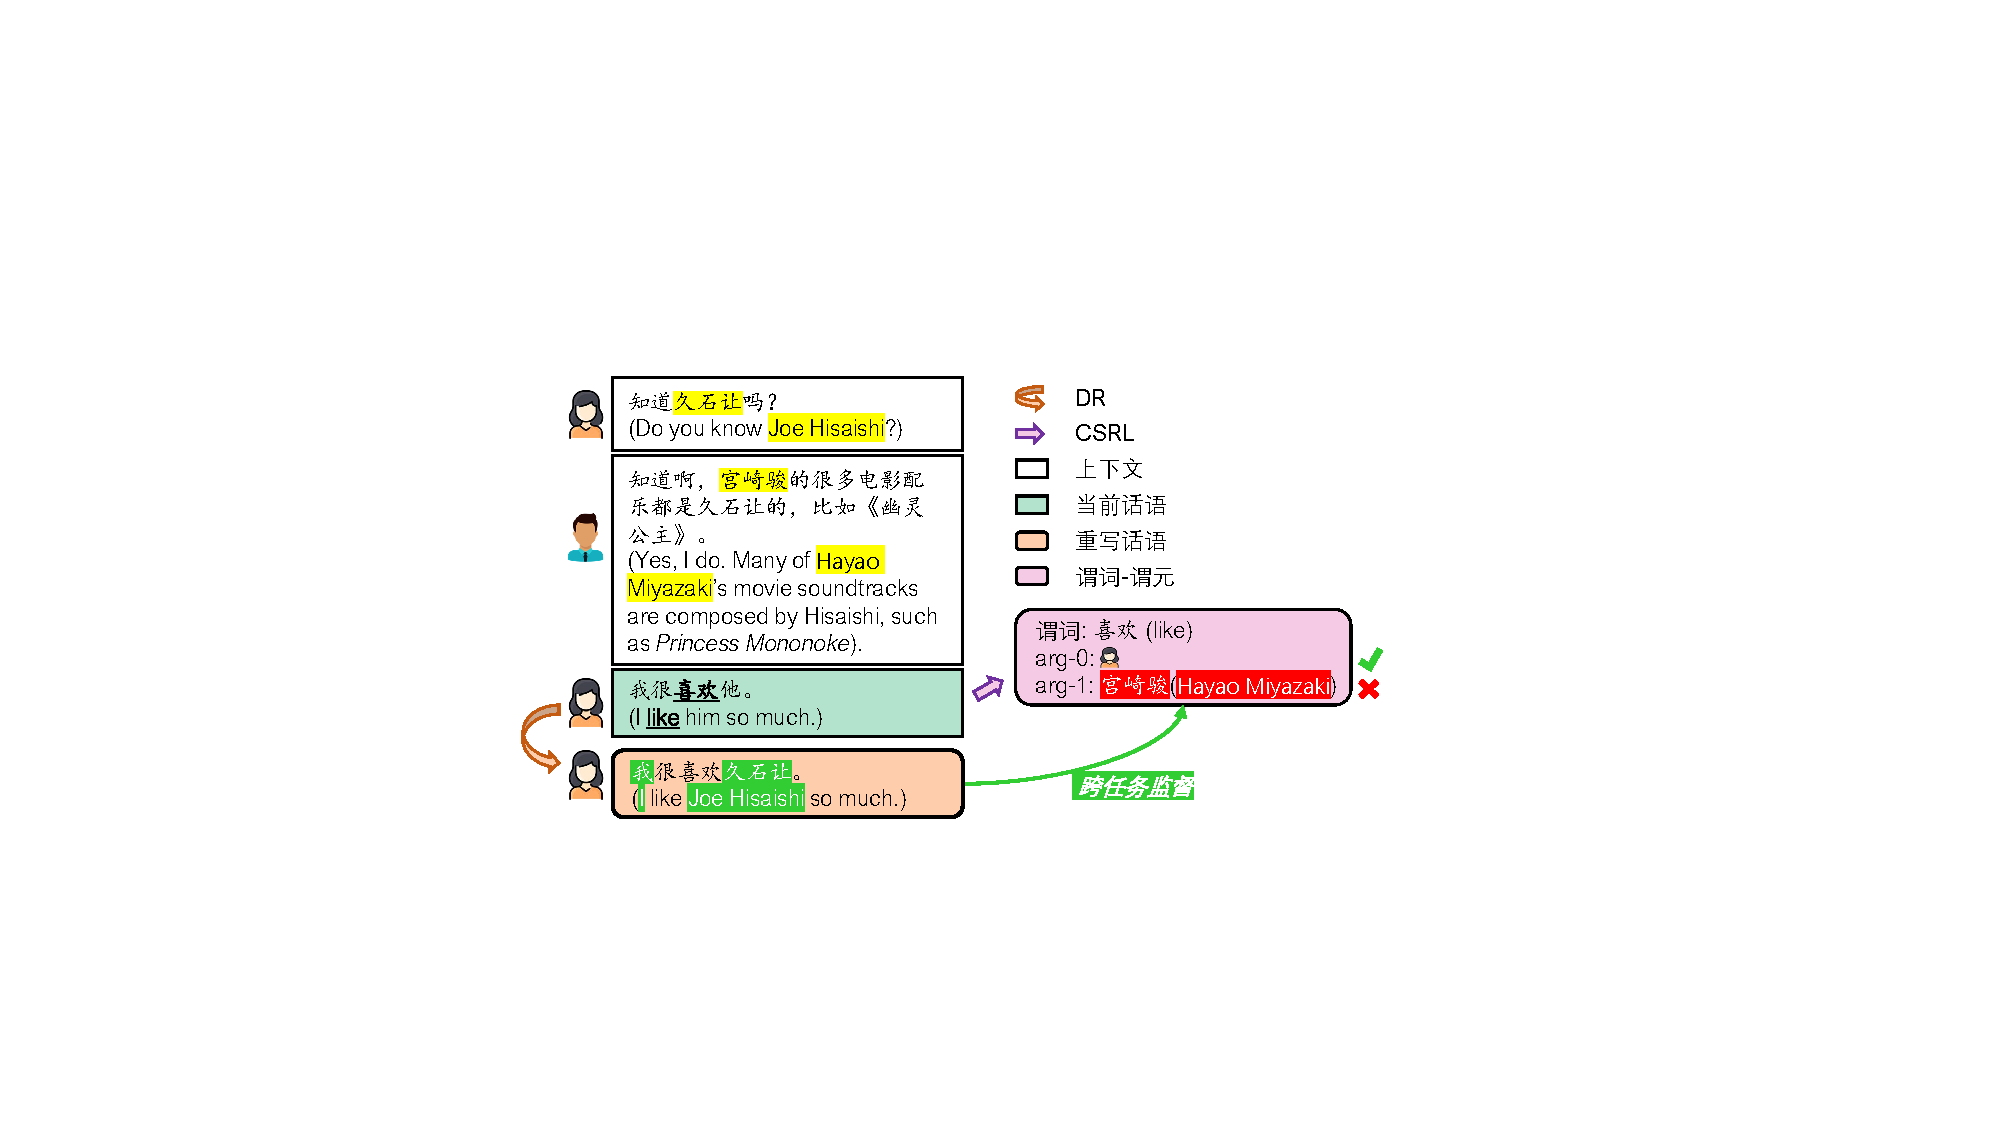
\includegraphics[width=0.7\textwidth]{pics/intro.pdf}
\caption{CSRL解析器和DR系统在对话中的跨任务监督示例。在重写话语中的\colorbox{LimeGreen}{\textcolor{white}{久石让}}对谓词“喜欢”的预测的\texttt{arg-1}产生了跨任务监督,同时\colorbox{LimeGreen}{\textcolor{white}{我}}对预测的\texttt{arg-0}产生了跨任务监督。}\label{fig:fdt_intro}
\end{figure}

在这项工作中,本章提出友邻训练,第一个跨任务的⾃训练框架。与单任务⾃训练相比,友邻训练利用友邻任务的监督来更好地选择伪标签。为了实现这个目标,友邻训练框架中包含两个新颖的模块:(1)翻译匹配器,它将每个实例的不同任务的伪标签映射到同⼀空间并计算匹配分数,代表来⾃不同任务的伪标签的跨任务匹配度;(2)增强(实例)选择器,它同时利⽤来自特定任务模型的伪标签的置信度和匹配分数来选择具有⾼质量伪标签的实例作为新的训练数据。本章选择CSRL和DR作为友邻任务来进⾏友邻训练的案例研究,并具体建模了在这两个任务之间实施友邻训练需要的翻译匹配器和增强选择器。域泛化和少样本学习的实验结果表明,友邻训练⼤⼤超过了一些经典和最先进的半监督学习算法。总的来说,本章的贡献包括:

\begin{itemize}
    \item 提出友邻训练,这是第一个跨任务⾃训练框架,利用友邻任务的监督在迭代训练过程中更好地选择伪标签。
    \item 提供了CSRL和DR之间实施友邻训练的具体方法,包括⼀个新颖的翻译匹配器和⼀个新颖的增强选择器。
    \item CSRL和DR的⼴泛实验证明了友邻训练的有效性,效果优于⼏个强基线方法,提升了模型理解对话中对话语义的能力。
\end{itemize}


\section{友邻训练框架}\label{sec:fdt_framework}

\subsection{自训练}
经典的⾃我训练旨在通过使⽤一小部分标注数据和⼤量无标注的数据迭代地改进单个任务的模型。在每次迭代中,模型⾸先为无标注数据打上伪标签。随后,选择一组带有伪标签的实例进行训练,这些实例理想情况下应该具有用于帮助模型泛化的信息。然后基于标签和伪标注数据上,最小化模型预测和标签的交叉熵以更新模型:

\begin{equation}\label{eq:loss}
    L = \sum_{i=1}^{N}y_{i}\log\frac{y_{i}}{p_{i}} + \lambda\sum_{i=1}^{N^{\prime}}y_{i}^{\prime}\log\frac{y_{i}^{\prime}}{p_{i}^{\prime}},
\end{equation}
其中左边项是标记数据的损失,右边是未标记数据的损失,⽽$\lambda$是平衡它们的系数;$N$($N^{\prime}$) 是实例数,$y$ ($y^{\prime}$)是标签,$p$ ($p^{\prime}$)是模型的输出概率。

⾃训练通常仅限于单项任务,但很多NLP任务是相关的。为一个任务训练的模型可以成为其他相关任务的好⽼师。本章通过引入⼩节\ref{sec:fdt}中介绍的两个新模块来探索自训练中的这种跨任务监督信号。

\subsection{友邻训练}\label{sec:fdt}
对于有两个任务的友邻训练\footnote{本章专注于两个任务之间的友邻训练,但是,友邻训练可以很容易地扩展到两个以上的任务。},有两个分别训练于数据集$\mathcal{L}_a$和$\mathcal{L}_b$的分类器$f_a$和$f_b$,它们分别的期望准确率是$\eta_a$和$\eta_b$。这两个数据集是独⽴创建的,两个任务的预测⽬标由⼀对翻译函数$\mathcal{F}_a: \hat{Y}_a \rightarrow \Sigma$和$\mathcal{F}_b: \hat{Y}_b \rightarrow \Sigma$产生关系,其中$\Sigma$是两个任务标签空间的子空间,$|\hat{Y}_a| \ge |\Sigma|, |\hat{Y}_b| \ge |\Sigma|$。我们规定翻译函数是一般的函数,产生一个具体翻译结果的期望概率是$\epsilon_{\mathcal{F}} = \frac{1}{|\Sigma|}$,并且,翻译函数是决定性,总是将来自不同任务的正确的预测结果对应到相同的翻译结果。

在迭代步$k$,两个分类器在无标注数据$\mathcal{U}$上进行预测,根据翻译函数的结果$\phi_a(x) =\mathcal{F}_a(f_a(x))$ and $\phi_b(x) =\mathcal{F}_b(f_b(x))$和一些筛选指标,比如相似度,一些拥有伪标签的实例$\mathcal{U}_\mathcal{F}^k$被选择作为新的训练数据。如果相似度被作为筛选指标,分类器$f_a$在这些例子上产生错误预测的概率是
\begin{align}
    &\mathrm{Pr}_{x} [f_a(x) \ne f^*_a(x)| \mathcal{\phi}_a(x) = \mathcal{\phi}_b(x)] \nonumber\\
     =& 1- \frac{\eta_a \mathrm{Pr}_{x} [ \mathcal{\phi}_a(x) = \mathcal{\phi}_b(x) | f_a(x) = f^*_a(x)] }{\mathrm{Pr}_{x} [\mathcal{\phi}_a(x) = \mathcal{\phi}_b(x)]},
\label{eq:error_rate}
\end{align}
其中$f^*$是最优的分类器。

由于训练数据,标注准则,模型以及预测目标等的不同,两个分类器区别很大,所以两个分类器很大几率是相互独立的,在这个条件下,等式~\ref{eq:error_rate}变成了

\begin{align}\label{eq:match_prob}
& 1- \frac{\eta_a (\eta_b + \epsilon_{\mathcal{F}} (1 - \eta_b) ) }{\mathrm{Pr}_{x} [\mathcal{\phi}_a(x) = \mathcal{\phi}_b(x)]} \nonumber \\
= & 1- \frac{Z}{Z + \eta_b\epsilon_{\mathcal{F}} (1 - \eta_a) + E},
\end{align}

其中$Z=\eta_a (\eta_b + \epsilon_{\mathcal{F}} (1 - \eta_b) )$,$E = \epsilon_\mathcal{F}^2(1-\eta_a)(1-\eta_b)$,这表明选出实例的数量和由于错误的翻译结果产生的错正例的数量$\eta_b\epsilon_{\mathcal{F}} (1 - \eta_a)$以及匹配的负例的数量$E$是负相关的。当选择具有足够大的目标空间$\Sigma$的翻译函数的时候,$\epsilon_\mathcal{F}$能够被最小化,这时如果两个分类器相符,选择错例的几率接近于0。同时也说明即使是$1-\eta_a$很大,即$f_a$表现很差,如果共同空间很大,选择错例的几率也能被控制得很小\footnote{直观上来看,如果共同空间很大,不同任务的独立的分类器产生相同但是错误的翻译结果的概率很小。}。当两个分类器之间的依赖逐渐增强,错例的概率同时也增加。当两个分类器完全依赖于对方的时候,等式\ref{eq:error_rate}变成了$1-\eta_a$,即经典的自训练框架。

基于这个公式,需要两个额外的模块:(1)一个将在不同任务上训练的两个模型的预测映射到同一空间并计算匹配分数的翻译匹配器;(2) 一个考虑到翻译预测的匹配分数和模型置信度的增强(实例)选择器,它为分类器选择具有伪标签的实例。

\noindent\textbf{翻译匹配器 } 给定两个友邻任务模型的预测$f_a(x)$和$f_b(x)$, 翻译匹配器$\mathcal{M}$利用翻译函数$\mathcal{F}_a$和$\mathcal{F}_b$得到翻译过的伪标签并且为这一对伪标签计算匹配分数$m$,表示它们在翻译空间中的相似度:
\begin{equation}\label{eq:matcher}
    m_{a,b}=\mathcal{M}\left(\mathcal{F}_a(f_a(x)),\mathcal{F}_b(f_b(x))\right),
\end{equation}
最大的匹配度是1,匹配分数作为筛选高质量伪标签的指标。

\noindent\textbf{增强选择器 } 除了伪标签相似性之外,还可以从模型置信度中找到有关伪标签质量的其他信息,来增强匹配分数。增强选择器同时考虑了来自任务模型的伪标签的置信度,记作$\left\{c_a,c_b \right\}$和匹配分数:
\begin{equation}\label{eq:selector}
    q_\tau = \mathcal{S}_\tau(m_{a,b}, c_\tau),
\end{equation}
其中$q_\tau \in \left\{0, 1\right\}$代表对于任务$\tau \in {a,b}$的伪标签选择结果。因此,拥有低匹配分数和高模型置信度的样例也可能被选择作为训练数据。

完整的算法如算法\ref{algo:framework}。

\begin{algorithm}[t]
    \SetKwInOut{Input}{Input}\SetKwInOut{Output}{Output}
    \Input{两个友邻任务的标注数据,$\mathcal{L}_a,\mathcal{L}_b$;无标注数据集合$\mathcal{U}$;任务模型$f_a,f_b$。}
    \Output{优化过后的$f_a,f_b$.}
    
    用 $\mathcal{L}_\tau$ $\left(\tau \in a,b\right)$预训练$f_\tau$;\\
    \While{模型尚未收敛}{
        $\mathcal{L}^{u}_a=\emptyset$; $\mathcal{L}^{u}_b=\emptyset$; \\
        \For{$z$ in $\mathcal{U}$} {
            生成$f_a(z),f_b(z)$和$c_a,c_b$;\\
            $m_{a,b}$ $\leftarrow$ 等式~\ref{eq:matcher};\\
            $q_a,q_b$ $\leftarrow$ 等式~\ref{eq:selector};\\
            \uIf{$q_\tau=1$ $\left(\tau \in a,b\right)$} {
                $\mathcal{L}^{u}_\tau = \mathcal{L}^{u}_\tau + \left\{z, v_\tau\right\}$;
            }
            % \uIf{$q_b=1$} {
            %     $\mathcal{L}^{u}_b = \mathcal{L}^{u}_b + \left\{z, v_b\right\}$;
            % }
        }
    根据等式~\ref{eq:loss}用 $\mathcal{L}_\tau,\mathcal{L}_{\tau}^u$更新$f_\tau$ $\left(\tau \in a,b\right)$;
    }
    返回$f_a,f_b$;
    \caption{两个任务的友邻训练}\label{algo:framework}
\end{algorithm}

\section{对话语义角色标注和对话重写之间的友邻训练}\label{sec:fdt_model}
为了验证友邻训练的有效性,本章选取对话语义角色标注(Conversational Semantic Role Labeling, CSRL)和对话重写(Dialogue Rewriting, DR)这两个对话理解作为友邻任务来进行友邻训练,进行案例研究。这两个任务都需要诸如共指和零代词解析等技能,同时这两个任务又侧重于对话话语的不
同属性:(1)CSRL 侧重于从整个对话历史中提取话语中谓词的谓元;(2) DR
旨在通过重写对话话语来恢复话语中的所有省略号和共指,使其与上下⽂⽆关且流畅。图~\ref{fig:fdt_overview}概述了上述两个任务之间的友邻训练。接下来,⾸先介绍任务模型,然后介绍用于友邻训练的翻译匹配器和增强选择器。

\begin{figure*}[ht]
\centering
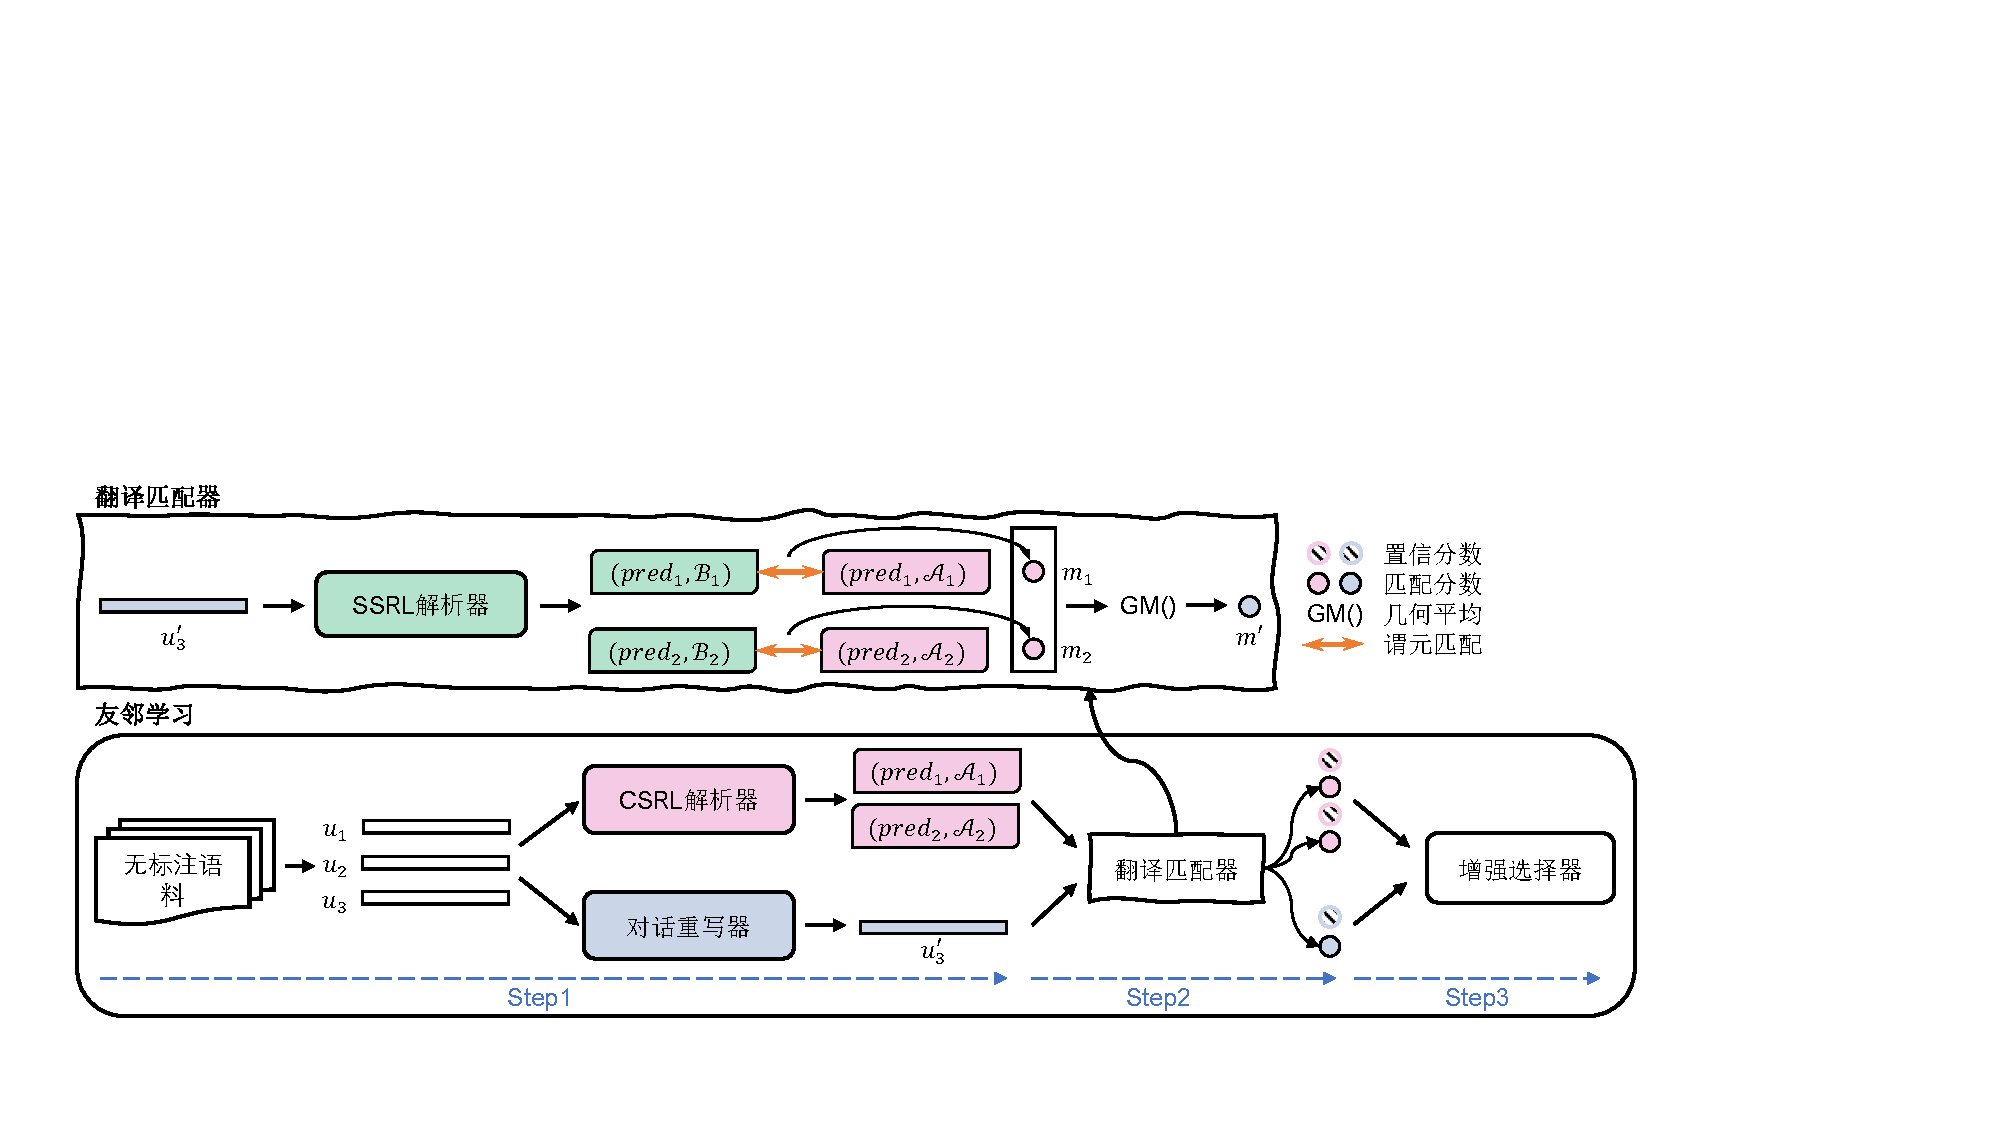
\includegraphics[width=\textwidth]{pics/overview_cn.pdf}
\caption{CSRL和DR之间友邻训练过程的概述。图中是一个对话实例,该实例具有三个话语,最后一个话语包含两个谓词。 Step1:未标记的对话由CSRL解析器和对话重写器标注,分别预测谓词(CSRL)的谓元和重写话语(DR)。Step2:两个任务的伪标签都被输入到翻译匹配器中以获得它们的匹配分数:翻译匹配器首先对重写的话语$u_3^{\prime}$进行句子级语义角色标注(Sentence-level Semantic Role Labeling, SSRL),然后比较结果与CSRL解析器的结果,并计算匹配分数。Step3:基于阈值的增强选择器根据置信度和匹配分数,最终决定是否将每个伪标签添加到训练数据中。}
\label{fig:fdt_overview}
\end{figure*}


\subsection{任务模型}
对话由$N$个按时间顺序排列的话语$\left\{u_1,...,u_N\right\}$ 组成。(1)给定话语$u_t$和$K$个谓词$\left\{\text{pred}_1,..., \text{pred}_K\right\}$ of $u_t$,CSRL解析器预测从对话中跨度作为所有谓词的谓元。(2)对话重写器根据上下文$\left\{u_1,...,u_{t-1}\right\}$重写$u_t$使其变成上下文无关的句子。

\noindent\textbf{对话编码器 } 本章将对话上下文$\left\{u_1,...,u_{t-1}\right\}$和当前话语 $u_t$拼接成一个长序列$\left\{x_1,...,x_M \right\}$并使用 BERT~\cite{devlin2018bert}对其进行编码以获得上下文嵌入:
\begin{equation}
   \mathbf{E} = \mathbf{e}_1, ..., \mathbf{e}_M=\textrm{BERT}(x_1,...,x_M) \in \mathbb{R}^{H \times M}. \nonumber
\end{equation}
CSRL和DR的编码器不共享任何参数,但为简单起见,本章对它们的输出使用相同的符号$\mathbf{E}$。

\noindent\textbf{对话语义角色标注 } 通过上下文嵌入,本章仿照~\citet{wu2021csagn}进一步生成谓词感知的话语表示$\mathbf{G} = \{\mathbf{g}_1, ..., \mathbf{g}_M\} \in \mathbb{R}^{H \times M}$:通过将自注意力~\cite{vaswani2017attention}应用到 $\mathbf{E}$ 并使用谓词感知掩码,其中符号只允许关注同一话语中的符号和包含谓词的话语中的符号:
\begin{equation}
\textrm{Mask}_{i,j} = 
    \begin{cases}
        1 & \text{if} \;u_{[i]} = u_{[j]} \; or \; u_{[j]} = u_{[pred]}, \\
        0 & \text{otherwise}, \nonumber
    \end{cases}
\end{equation}
其中 $u_{[m]}$ 表示包含标记 $x_m$ 的话语,$u_{[pred]}$ 表示带有谓词的话语。

然后通过前馈网络投射谓词感知表示以获得每个符号的标签分布:
\begin{equation}
    \mathbf{P}^c=\textrm{softmax}_{\textrm{column-wise}}(\mathbf{W}_c\mathbf{G} + \mathbf{b}_c) \in \mathbb{R}^{C \times M}, \nonumber
\end{equation}
其中 $\mathbf{W}_c$ 和 $\mathbf{b}_c$ 是可学习的参数,$C$ 是标签的数量。 标签遵循 BIO 序列标签方案:B-X 和 I-X 分别表示符号是谓元X的第一个符号和内部的符号,其中 O 表示符号不属于任何谓元。CSRL 解析器对$K$个谓词的输出表示为 $\left\{\mathcal{A}_1, ..., \mathcal{A}_K\right\}$,其中集合 $\mathcal{A} _k$ 包含 $\text{pred}_k$ 的谓元。

\noindent\textbf{对话重写 } 仿照 \citet{hao2021rast},我们将 DR 转换为序列标注任务。 具体来说,$\mathbf{E}$ 顶部的二元分类器首先确定是否在重写的话语中保留话语 $u_t$ 中的每个符号:
\begin{equation}
    \mathbf{P}^d=\textrm{softmax}_{\textrm{column-wise}}(\mathbf{W}_d\mathbf{E} + \mathbf{b}_d) \in \mathbb{R}^{2 \times M}, \nonumber
\end{equation}
其中 $\mathbf{W}_d$ 和 $\mathbf{b}_d$ 是可学习的参数。 接下来,预测是否在每个符号前面插入一段上下文跨度。 在实践中,采用两个自注意力层~\cite{vaswani2017attention}来计算对话中作为待插入跨度的开始索引或结束索引的概率:
\begin{align}
    \mathbf{P}^{st} &= \textrm{softmax}_{\textrm{column-wise}}(\textrm{Attn}_{st}(\mathbf{E})) \in \mathbb{R}^{M \times M}, \nonumber \\
    \mathbf{P}^{ed} &= \textrm{softmax}_{\textrm{column-wise}}(\textrm{Attn}_{ed}(\mathbf{E}))\in \mathbb{R}^{M \times M}, \nonumber
\end{align}
其中 $\mathbf{P}^{st}_{i,j}$ ($\mathbf{P}^{ed}_{i,j}$) 表示 $x_i$($x_j$) 是跨度的开始(结束)索引的概率。 然后通过将 argmax 应用于 $\mathbf{P}$,可以获得每个符号的跨度的开始和结束索引:
\begin{align}
    \mathbf{s}^{st} = \textrm{argmax}_{\textrm{column-wise}}(\mathbf{P}^{st}) \in \mathbb{R}^{M}, \nonumber \\
    \mathbf{s}^{ed} = \textrm{argmax}_{\textrm{column-wise}}(\mathbf{P}^{ed}) \nonumber \in \mathbb{R}^{M},
\end{align}
在$x_m$前面插入的跨度的概率是$\mathbf{P}^{st}_{\mathbf{s}_m^{st},m} \times \mathbf{P}^{ed }_{\mathbf{s}_m^{ed},m}$,其中 $\mathbf{s}_m^{st} \leqslant \mathbf{s}_m^{ed}$。 当$\mathbf{s}_m^{st} > \mathbf{s}_m^{ed}$时,表示没有插入。 $u_t$ 的对话重写器的输出表示为 $u_t^{\prime}$。

\subsection{翻译匹配器}
为了翻译来自 CSRL 解析器 $\left\{\mathcal{A}_1, ..., \mathcal{A}_K\right\}$ 和对话重写器 $u_t^{\prime}$ 的输出(伪标签)到同一个空间,我们利用参数固定的普通句子级语义角色解析器贪婪地从重写的话语 $u_t^{\prime}$ 中为$K$个谓词提取谓元,表示为 $\left\{\mathcal{B}_1, ..., \mathcal{B}_K\right\}$(表~\ref{tab:fdt_case} 展示了一个例子)。所以公共目标空间 $\Sigma$ 是 CSRL 的标签空间,它足够大,可以使所选实例的错误率保持在很低的水平(见小节~\ref{sec:fdt}的分析)。$\text{pred}_k$ 的匹配分数 $m_{k} \in [0,1]$ 是根据 $\mathcal{A}_k$ 和 $\mathcal{B}_k$ 之间的编辑距离计算的:
\begin{equation}
    m_{k} = 1 - \frac{\textrm{dist}(\oplus \mathcal{A}_k, \oplus \mathcal{B}_k)}{\textrm{max}(\textrm{len}(\oplus \mathcal{A}_k), \textrm{len}(\oplus \mathcal{B}_k))}, \nonumber
\end{equation}
其中 dist() 计算两个字符串之间的编辑距离,\textrm{len()} 返回字符串的长度,$\oplus \mathcal{A}_k$ 表示集合 $\mathcal{A}_k$ 中的谓元按照预定义的谓元顺序拼接\footnote{谓元拼接顺序:\texttt{ARG0}, \texttt{ARG1}, \texttt{ARG2}, \texttt{ARG3}, \texttt{ARG4}, \texttt{ARGM-TMP }, \texttt{ARGM-LOC}, \texttt{ARGM-PRP}}(空字符串表示谓元不存在)。此外,我们为重写的话语 $u_t^{\prime}$ 按如下计算匹配分数 $m^{\prime} \in [0,1]$:
\begin{equation}
    m^{\prime} = \textrm{GM}(m_1,...,m_K), \nonumber
\end{equation}
其中GM()表示几何平均。

\subsection{增强选择器}
增强选择器根据匹配分数和置信度选择高质量的伪标签。 对于 CSRL,我们根据 softmax 层的输出计算每个谓词的置信度分数。具体来说,我们通过乘以其符号的概率来获得 $\text{pred}_k$ 的谓元的置信度,表示为 $\{a_{k1}, ..., a_{k|\mathcal{A}_k |}\}$。 然后,我们使用属于 $\text{pred}_k$ 的参数的所有置信度的几何平均值作为 $\text{pred}_k$ 的置信度。 $\text{pred}_k$ 的总分 $s_{k} \in [0,1]$ 计算如下:
\begin{equation}
    s_k = \alpha \textrm{GM}(a_{k1}, ..., a_{k|\mathcal{A}_k|}) + (1 - \alpha) m_{k},\nonumber
\end{equation}
其中超参数 $\alpha$ 用于平衡匹配分数和置信度。对于 DR,我们将要插入的跨度和决定是否保留符号的概率相乘作为 $u_t^{\prime}$ 的模型置信度,表示为 $b_{t}$。 $u_t^{\prime}$的总分$r_t \in [0,1]$如下:
\begin{equation}
    r_t = \beta b_t + (1 - \beta)m^{\prime},\nonumber
\end{equation}
其中,超参数 $\beta$ 的值越大,模型的置信度就越重要。 $\alpha$ 和 $\beta$ 在实验中的两个任务都设置为 0.2。

为了进行伪标签筛选,对 $s_k$ 和 $r_t$ 设置了选择阈值,以控制所选伪标签的数量和质量。 本章在小节~\ref{sec:abl}中分析了不同阈值的影响。

\section{实验}\label{sec:fdt_exp}
\subsection{设置}
\noindent\textbf{数据集 } 本章的实验在电影、名人、书评、产品和社交网络等领域的实验中使用了五个对话数据集。对于 CSRL,使用 DuConv~\cite{xu2021conversational} 和 WeiboCSRL,对于 DR,使用 REWRITE~\cite{su2019improving} 和 RESTORATION~\cite{pan2019improving}。 同一任务的数据集在域和大小上不同。 WeiboCSRL 是一个新注释的 CSRL 数据集,用于跨领域测试目的。 此外,使用 LCCC-base~\cite{wang2020large} 作为无标注语料库,这是一个大型中文对话数据集,包含来自各种社交媒体的 79M 严格清洗的对话。

\noindent\textbf{WeiboCSRL标注流程 } 用于CSRL标注的对话是从LCCC-base~\cite{wang2020large}中提取的,它至少包含4个对话话语,80个字符,以确保CSRL和DR有足够的上下文。 这些对话和在小节~\ref{sec:fdt_exp}用作实验的无标注数据的对话来自LCCC-base 的不同部分。对于每个对话,在Chinese Proposition Bank\footnote{\url{https://verbs.colorado.edu/chinese/cpb/}}框架文件的指导下,对最后一句话中的谓词进行标注。对于每个谓词,标注的参数是核心谓元 \texttt{ARG0-ARG4} 和附加词 \texttt{ARGM-LOC}、\texttt{ARGM-MNR}、\texttt{ARGM-TMP} 和 \texttt{ARGM-NEG},其定义见~\cite{xue2006semantic}。 \texttt{ARGM-MNR} 未包含在小节~\ref{sec:fdt_exp}进行标注,因为 \texttt{ARGM-MNR} 的注释在 DuConv(CSRL 的训练数据)中缺失。 最终获得了3891个带注释的谓词。

\noindent\textbf{数据集详情 } 表~\ref{tab:fdt_dataset} 显示了实验中使用的数据集的统计数据。 DuConv~\cite{xu2021conversational} 专注于电影和名人,实验中采用与 \citet{xu2021conversational} 相同的训练/开发/测试集拆分。 REWRITE~\cite{su2019improving} 包含从中国社交媒体平台爬取的20K对话,主题广泛;每个对话的最后一句话被重写以恢复所有共指和遗漏的信息。RESTORATION~\cite{pan2019improving}包含来自豆瓣\footnote{\url{https://www.douban.com}}的对话,大部分为书评、影评或商品评论。与REWRITE相比,它包含更多带标注的对话,但大约40\%的最后话语不需要重写。
\begin{table}[!ht]
    \centering
    \caption{数据集统计信息。}
    \label{tab:fdt_dataset}
    \resizebox{0.7\textwidth}{!}{
    \begin{tabular}{llr}
        \toprule
         & \textbf{领域} & \textbf{\#样例(训练/开发/测试)} \\
         \midrule
        \textbf{DuConv} & 电影和明星 & 23361 / 2852 / 2977 \\
        \textbf{WeiboCSRL} & 社交媒体 & - / 1945 / 1946 \\
        \textbf{REWRITE} & 社交媒体 & 16925 / 1000 / 1000 \\
        \textbf{RESTORATION} & \makecell{书评、影评、产品评价} & - / 5000 / 5000 \\
        \bottomrule
    \end{tabular}
    }
\end{table}

\noindent\textbf{实验场景 }
主要实验涉及两种场景。(1)域泛化(Domain Generalization,DG):使用DuConv作为源域的训练数据,WeiboCSRL用于域外评估,而对于DR,REWRITE用于训练,RESTORATION用于评估。
(2)少样本学习(Few-shot learning,FSL):分别从 DuConv 和 REWRITE 中随机抽取 100 个案例作为 CSRL 和 DR 的训练数据,并进行域内评估,这意味着这两个任务的模型只用少量的样本进行联合训练。 两种场景的未标记数据都是从 LCCC-base 中提取的 20k 对话。实验场景任务的数据集配置如表~\ref{tab:apx_scenario}所示。

\noindent\textbf{预处理细节 } 输入对话的最大长度设置为125。将DuConv的基于词的标注转换为基于字符的标注,转换脚本\footnote{\url{https://github .com/freesunshine0316/RaST-plus}} 由 \citet{hao2021rast} 提供。并将DR的基于词表示的标签转换成基于符号的标签。对于无标注数据,丢弃少于4轮的对话以保证对话有足够的上下文。

\noindent\textbf{模型 } 使用预训练的 BERT\footnote{\url{https://huggingface.co/bert-base-chinese}}~\cite{devlin2018bert} 作为 CSRL 和 DR 的对话编码器。 超参数 $\alpha$ 和 $\beta$ 的值都设置为 0.2,选择阈值设置为 0.6。 翻译匹配器中使用了最先进的句子级语义角色标记 (SSRL) 解析器\footnote{\url{https://github.com/hankcs/HanLP}},其结构与\cite{he-choi-2021-stem}相似。

\noindent\textbf{训练细节 } 实验中采用 AdamW~\cite{loshchilov2017decoupled} 优化器、学习率 4e-5、批大小16来优化模型。并使用 $\lambda=1$ 来平衡标记和未标记数据的损失。

\begin{table}[ht]
    \centering
    \caption{域泛化和少样本学习的数据集配置。}
    \label{tab:apx_scenario}
    \resizebox{0.7\textwidth}{!}{
    \begin{tabular}{llll}
        \toprule
        & \textbf{任务} & \textbf{训练} & \textbf{开发\&测试} \\
        \midrule
        \textbf{\multirow{2}{*}{\makecell{DG}}} & CSRL & DuConv (train) & WeiboCSRL (dev,test) \\
        \cmidrule(lr){2-4}
        & DR & REWRITE (train) & RESTORATION (dev,test) \\
        \midrule
        \textbf{\multirow{2}{*}{\textbf{FSL}}} & CSRL & DuConv (100个样本) & DuConv (dev,test) \\
        \cmidrule(lr){2-4}
        & DR & REWRITE (100个样本) & REWRITE (dev,test) \\
        \bottomrule
    \end{tabular}
    }
\end{table}

\noindent\textbf{验证方法 } 按照~\citet{wu2021csagn} 报告 CSRL 谓元的精度(Pre.)、召回率(Rec.)和 F1;按照~\citet{hao2021rast} 报告单词错误率(WER)~\cite{morris2004and}, Rouge-L (R-L)~\cite{lin2004rouge} 和 DR 的句子级精确匹配 (EM) 百分比。

\subsection{基线}\label{sec:baseline}
本章的实验将友邻训练与六种半监督训练范式进行比较:两种经典方法,例如标准自训练 (SST)~\cite{scudder1965probability} 和标准协同训练 (SCoT)~\cite{blum1998combining},以及四种最先进的方法,如均值教师 (MT)~\cite{tarvainen2017mean}、交叉伪监督 (CPS)~\cite{chen2021semi}、批量重新加权自训练 (STBR)~\cite{bhat2021self} 和自学习 (STea )~\cite{yu2021self}。 标准自训练~\cite{scudder1965probability} 使用基本模型为未标记数据生成伪标签,并使用它们训练新的基本模型,重复直到收敛。 标准协同训练~\cite{blum1998combining} 类似于标准自训练,但是有两个不同的基础模型处理相同的任务,生成伪标签并添加可信的样例用于迭代训练。均值教师~\cite{tarvainen2017mean} 动态维护一个教师模型,其权重是学生模型在迭代中权重的指数移动平均值。 交叉伪监督~\cite{chen2021semi},一种最先进的自训练的变体,维护两个具有不同初始化的网络;一个网络的伪标签用于监督另一个网络。 批量重新加权自训练~\cite{bhat2021self} 是一种最先进的自训练方法,在训练时根据教师模型的置信度对批量伪标签进行重新加权。 自学习~\cite{yu2021self},一种最先进的半监督方法,按顺序训练一名初级教师、一名高级教师和一名专家学生来利用无标注的数据。

对于基线的超参数,保留了与提出的方法相同的通用超参数,例如学习率、批量大小、优化器等。 并且采用了原始论文中使用的方法特定超参数的值,例如自学习中软硬标签的合并权重和平均教师更新的平滑参数。

\begin{table*}[ht]
\caption{域泛化和少样本学习的测试结果。 Base 表示使用来自单个任务的数据训练的任务模型。 Multitask-Base 表示 CSRL 和 DR 共享相同对话编码器的基础模型。结果取三次相同实验的平均值。 $\Downarrow$ 表示越低越好。 对于少样本学习,表中提供了使用单个任务的完整训练集训练的基础模型的性能以供参考。}
\label{tab-main}
\begin{subtable}{1.0\textwidth}
    \centering
    \caption{使用 DuConv 和 REWRITE 训练的模型的域泛化结果。}
    \resizebox{0.9\textwidth}{!}{

    \begin{tabular}{lcccccc}
    \toprule
    
    {} & \multicolumn{3}{c}{WeiboCSRL} & \multicolumn{3}{c}{RESTORATION}  \\
    
    \cmidrule[0.5pt](rl){2-4}
    \cmidrule[0.5pt](rl){5-7}

    {\textbf{方法}} & {\textbf{Pre.}} & {\textbf{Rec.}} & {\textbf{F1}} & {\textbf{R-L}} & {\textbf{EM}} & {\textbf{WER}($\Downarrow$)} \\
    \midrule
    Base & 57.97 & 54.47 & 56.16 & 82.78 & 25.25 & 28.69  \\
    Multitask-Base & 53.66 & 54.32 & 53.99 & 81.68 &  22.49 & 32.44 \\
    SST~\cite{scudder1965probability} & 60.85 & 56.54 & 58.62 & 85.22 & 32.97 & 22.22  \\
    MT~\cite{tarvainen2017mean} & 58.42 & 55.71 & 57.03 & 83.76 & 28.82 & 26.49 \\
    CPS~\cite{chen2021semi} & 60.34 & 52.87 & 56.36 & 85.60 & 32.68 & 22.78 \\
    SCoT~\cite{blum1998combining} & 57.33 & 54.13 & 55.69  & 84.51 & 29.25 & 24.87 \\
    STBR~\cite{bhat2021self} & 60.77 & 58.04 & 59.38  & 85.79 & 33.78 & 23.30 \\
    STea~\cite{yu2021self} & 60.10 & 55.13 & 57.50  & 85.75 & 34.23 & 22.17  \\
    \midrule
    FDT (Ours) & \textbf{\makecell{65.29($\uparrow$4.44)}} & \textbf{\makecell{58.63($\uparrow$2.09)}} & \textbf{\makecell{61.78($\uparrow$3.16)}} & \textbf{\makecell{86.82($\uparrow$1.60)}} & \textbf{\makecell{38.22($\uparrow$5.25)}} & \textbf{\makecell{20.31($\uparrow$1.91)}} \\
    \bottomrule
    \end{tabular}
    }
    \end{subtable}
    %
\vspace*{0.3 cm}
\newline    %
    \begin{subtable}{1.0\textwidth}
    \centering
    \caption{使用 DuConv 和 REWRITE 训练的模型的小样本学习结果。}
    \resizebox{0.9\textwidth}{!}{
    \begin{tabular}{lcccccc}
    \toprule
    % {} &  \multicolumn{6}{c}{\textbf{Few-shot Learning}} \\
    
    % \cmidrule[0.5pt](rl){2-7}
    
    {} & \multicolumn{3}{c}{DuConv} & \multicolumn{3}{c}{REWRITE} \\
    
    \cmidrule[0.5pt](rl){2-4}
    \cmidrule[0.5pt](rl){5-7}

    {\textbf{方法}} & {\textbf{Pre.}} & {\textbf{Rec.}} & {\textbf{F1}} & {\textbf{R-L}} & {\textbf{EM}} & {\textbf{WER}($\Downarrow$)} \\
    \midrule
    Base & 29.50 & 21.90 & 25.14 & 73.44 & 3.60 & 39.98 \\
    Multitask-Base & 22.43 & 20.63 & 21.49 & 78.97 & 11.70 & 40.46 \\
    SST~\cite{scudder1965probability}  & 34.16 & 27.49 & 30.46 & 80.93 & 27.80 & 31.02 \\
    MT~\cite{tarvainen2017mean} & 36.32 & 30.69 & 33.27 & 81.66 & 33.00 & 31.66 \\
    CPS~\cite{chen2021semi} & 37.14 & 29.47 & 32.86 & 79.56 & 23.30 & 32.60 \\
    SCoT~\cite{blum1998combining} & 38.37 & 26.15 & 31.10 & 78.58 & 22.31 & 33.79 \\
    STBR~\cite{bhat2021self} & 32.37 & 25.21 & 28.34 & 82.37 & 29.80 & 30.31 \\
    STea~\cite{yu2021self} & 39.34 & 28.78 & 33.25 & 83.04 & 31.57 & 30.36 \\
    \midrule
    FDT (Ours) & \textbf{\makecell{40.41($\uparrow$6.25)}} & \makecell{30.82($\uparrow$3.33)} & \makecell{34.97($\uparrow$4.51)} & \makecell{82.83($\uparrow$1.90)} & \makecell{34.20($\uparrow$6.40)} & \makecell{27.87($\uparrow$3.15)} \\
    FDT-S (Ours) & 40.12 & \textbf{33.41} & \textbf{36.46}  & \textbf{83.11} & \textbf{37.10} & \textbf{26.88} \\
    \midrule
    \textit{\textbf{Fully-trained} Base} & \textit{69.83} & \textit{68.53} & \textit{69.17} & \textit{89.47} & \textit{52.30} & \textit{20.54} \\
    \bottomrule
    \end{tabular}
    }
    \end{subtable}
\end{table*}


\subsection{主要结果}
表 ~\ref{tab-main} 显示了友邻训练(Friend-training, FDT)和小节~\ref{sec:baseline}中提到的基线之间的比较。 FDT 在域泛化和少样本学习场景中均以显著优于基线,达到最佳,这证明了 FDT 在不同实验情况下有效地利用大规模无标注语料库。 此外,箭头$(\uparrow)$ 中展示了 FDT 相对于 SST 的性能提升。在少样本学习场景下,FDT 在 DuConv 的 F1 和 REWRITE 的 WER 上分别比 SST 提高了 4.51 和 3.15 的绝对点数,比域泛化的 3.16 和 1.91 点都高,表明 FDT 在少样本学习中的有更高的潜力。此外,对于少样本学习,实验中进一步考虑了可以使用来自友邻任务的完整训练基础模型的情况,表示为 FDT-S。如表~\ref{tab-main},当目标任务是 CSRL 时,FDT-S 在 F1 上比 FDT 高出 1.49 个点,当目标任务是 DR 时,FDT-S 在 WER 上比 FDT 高出 0.99 个点,在 EM 上比 FDT 高出 2.90 个点,这表明来自友邻任务的更可靠的监督可以进一步增强目标任务的少样本学习。


\subsection{分析}\label{sec:abl}
我们进行实验来分析所选参数和设置如何与 FDT 中的模型性能相互作用。

\noindent\textbf{选择阈值 } 在域泛化场景中改变 CSRL 和 DR 的选择阈值并跟踪模型性能:将朋友任务的选择阈值固定为最佳,当改变评估任务时。 如图 \ref{fig:thres} 所示,当阈值逐渐增加时,模型变得更好,CSRL 的 F1 更高,DR 的 WER 更低。 此现象可以归因于错误的伪标签被 FDT 的增强选择器过滤掉了。 然后模型性能达到峰值并随着阈值在高值区间不断增加而下降,这是由于高阈值产生的伪标签数量不足以进行迭代训练。 自动选择合适的选择阈值值得在未来探索。

\noindent\textbf{基础模型的强度 } 为了理解和比较友邻训练或自训练的基础模型的性能如何影响它们的最终性能,在评估域外测试时比较了拥有在源域中不同百分比的标记数据上训练的基础模型的STBR、STea 和 FDT三种方法。具体来说,实验遵循域泛化设置并使用可变百分比的标注数据来进行实验。

对于CSRL和DR,分别设置标注数据量为\{10\%/10\%, 30\%/30\%, ..., 90\%/90\%\}。结果如图~\ref{fig:tea_csrl}和图~\ref{fig:tea_rewr}所示。 可以看到,无论是给定弱基础模型还是强基础模型,所有采用自训练来利用无标注数据的方法都大大超过了基础模型,证明了自训练范式的有效性。此外,FDT在评估标注数据的百分比方面取得了最好的结果:当基础模型具有大量训练数据时,例如用30\%标注数据及以上训练模型时,FDT 的性能明显优于 STBR 和 STea,证明 FDT 通过跨任务监督能够更有效地利用从标注数据中学习到的特征。

\noindent\textbf{共同更新的作用 } 本小节探讨了友邻任务的其中一个模型已完全训练且不必更新的情况。假设FDT-SF是FDT 具有固定的从领域泛化中的友邻任务完全训练的基础模型\footnote{具体来说,当评估任务是CSRL时,两个任务的标注数据量设置为\{10\%/100\%, 30\%/100\%, 50\%/100\%, 70\%/100\%, 90\%/100\%\},评估任务为DR时 , 设置为\{100\%/10\%, 100\%/30\%, 100\%/50\%, 100\%/70\%, 100\%/90\%\}.}。 如图~\ref{fig:fixabl} 所示,由于友邻任务的强监督,FDT-SF 在为评估任务提供弱基础模型时优于 FDT。 然而,当评估任务被赋予一个训练有素的模型时,FDT 优于 FDT-SF,这证明了在友邻训练中共同更新模型的好处。


\begin{figure*}[!htbp]
\centering
    \begin{subfigure}[t]{0.31\textwidth}
    \centering
    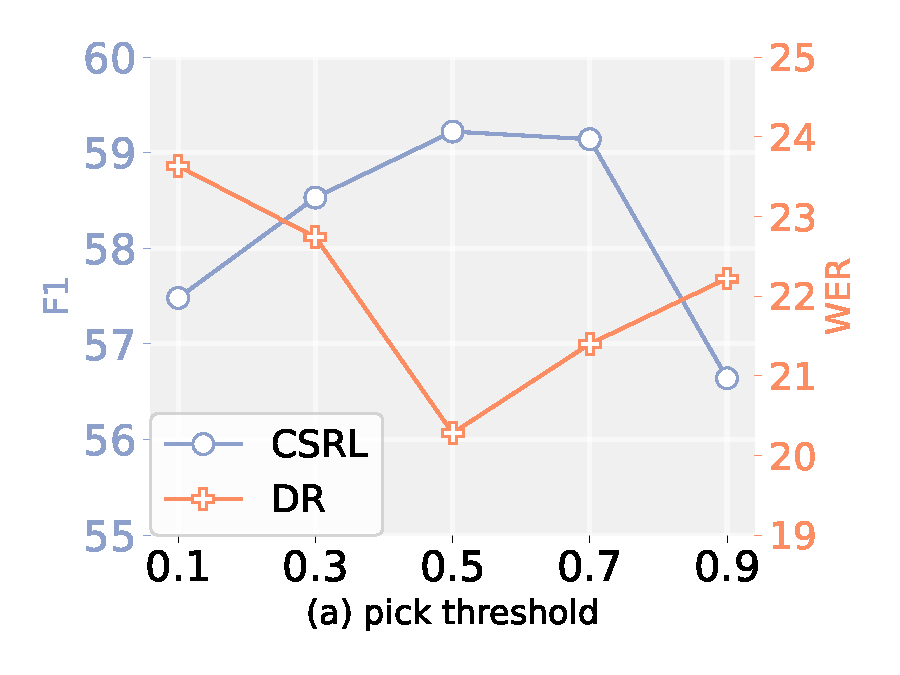
\includegraphics[width=\textwidth]{pics/abla_pick_threshold.pdf}
    \caption{选择阈值的影响。}\label{fig:thres}
    \end{subfigure}
    \quad
    \begin{subfigure}[t]{0.31\textwidth}
    \centering
    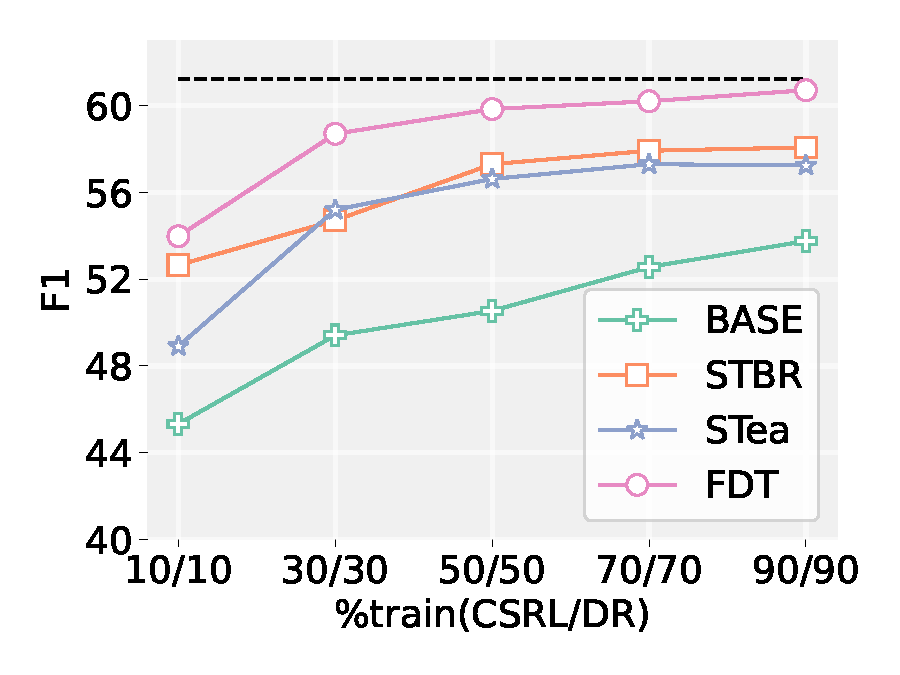
\includegraphics[width=\textwidth]{pics/abla_initial_teacher_csrl.pdf}
    \caption{CSRL在测试集上F1。}\label{fig:tea_csrl}
    \end{subfigure}
    \quad
    \begin{subfigure}[t]{0.31\textwidth}
    \centering
    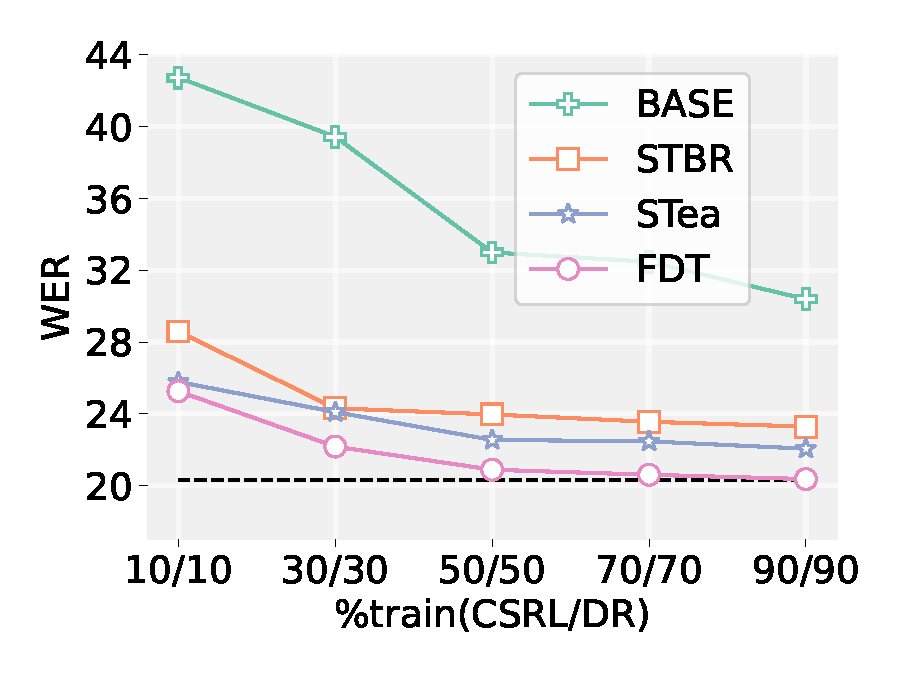
\includegraphics[width=\textwidth]{pics/abla_initial_teacher_rewr.pdf}
    \caption{DR在测试集上的WER。}\label{fig:tea_rewr}
    \end{subfigure}

\caption{子图(b)和(c)显示了比较方法在不同基础模型强度下的模型性能; 水平虚线表示 FDT 具有完全训练的基础模型的性能。}
\end{figure*}

\begin{figure}[!htbp]
\centering
    % \begin{subfigure}[b]{0.55\textwidth}
    \centering
    \subfloat[CSRL测试集上的性能。]
    {
    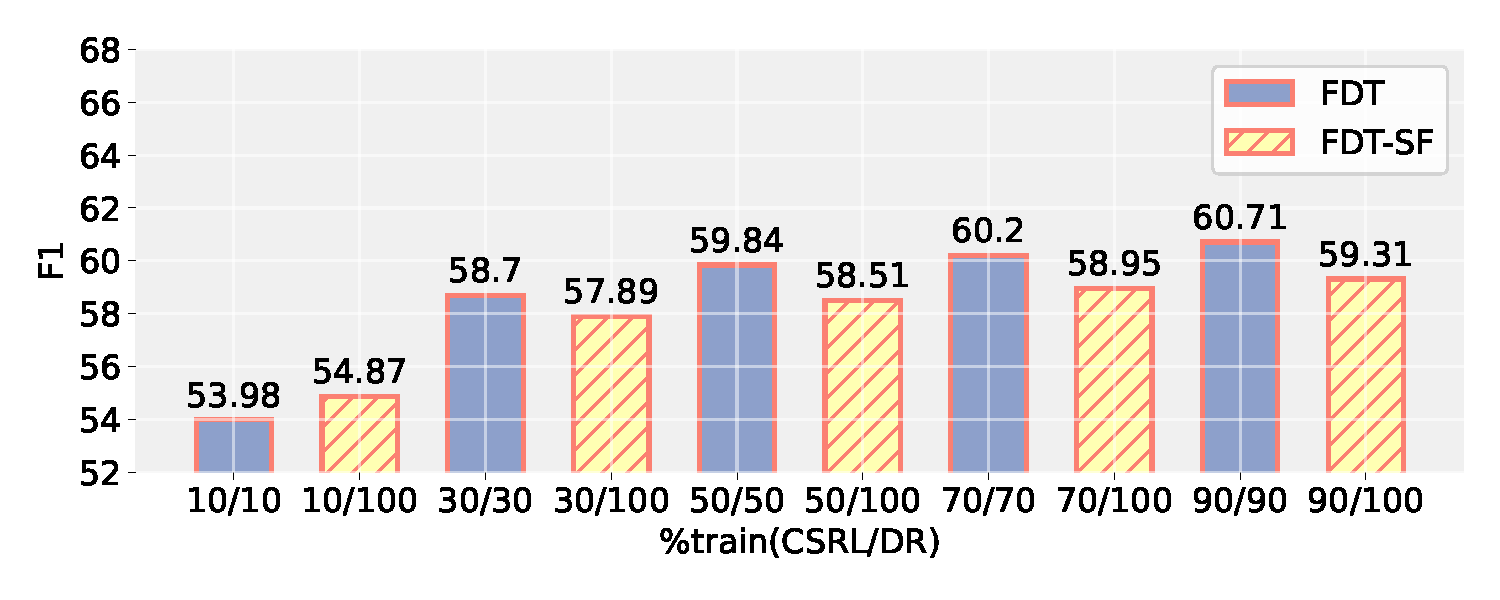
\includegraphics[width=0.47\textwidth]{pics/abla_fixtea_csrl.pdf}
    }
    % \caption{CSRL测试集上的性能。}
    % \end{subfigure}
    \quad
    % \vspace{2cm}
    % \begin{subfigure}[b]{0.55\textwidth}
    \centering
    \subfloat[DR 测试集上的性能。]
    {
        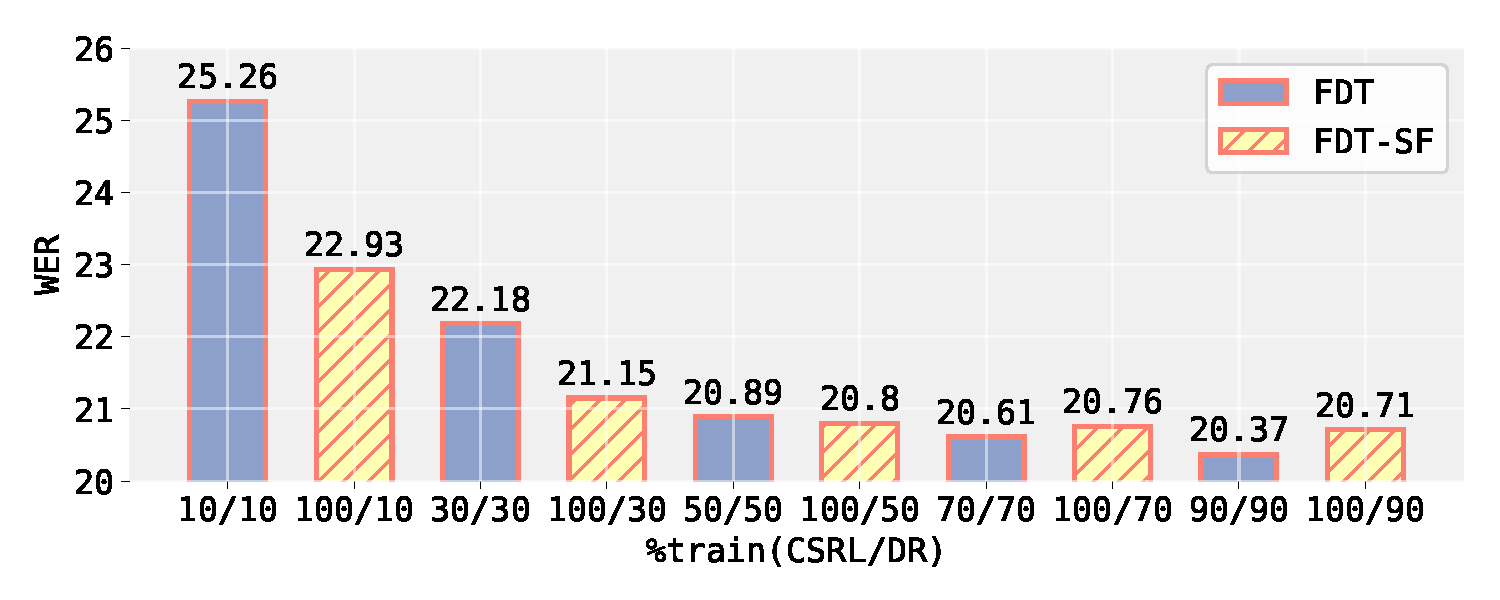
\includegraphics[width=0.47\textwidth]{pics/abla_fixtea_rewr.pdf}
    }
    % \caption{DR 测试集上的性能。}
    % \end{subfigure}
\caption{共同更新在友邻训练中的作用。}\label{fig:fixabl}
\end{figure}

\subsection{案例研究}\label{sec:fdt_case}
表~\ref{tab:fdt_case}展示了一个选择伪标签的代表性案例。 当前话语中有两个谓词:“是”和“受”。 对于“是”,CSRL 解析器生成了 ARG1,而 SSRL 解析器根据重写的话语给出相同的 ARG1,但还有 ARG0。由于谓元的不同,所以整体得分不高,如果设置高的选择阈值,这个谓词可以被认为是低质量的。对于“受”,CSRL 和 SSRL 解析器给出相同的参数,这是正确的答案。但是,如果我们只考虑谓词的模型置信度,即0.54,而不是考虑整体得分,即0.90,那么这个高质量的谓词更有可能被丢弃,并且重写后的话语能够获得了很高的总分,这也是所期望的。
\begin{table*}[t!]
\centering
\caption{案例研究:[A] 和 [B] 是说话者的签名。 ch 和 en 是语言缩写。}
\label{tab:fdt_case}
\resizebox{\textwidth}{!} {
    \begin{tabular}{lll}
    \toprule
    对话历史 
    &
    \multicolumn{2}{l}{\makecell[l]{ch: [A]我有一个非常喜欢的女明星。[B]她叫什么名 字?[A]布蕾克·莱弗利。[B]她很有名吗?\\ en: [A] I have a favorite actress. [B] What's her name? [A] Blake Lively. [B] Is she famous?}} \\
    \midrule
    当前话语
    & 
    \multicolumn{2}{l}{\makecell[l]{ch: [A]她是一个非常受关注的女明星。\\en: [A] She is a actress attracting much attention.}} \\
    \midrule
    重写话语
    &
    \multicolumn{2}{l}{\makecell[l]{ch: [A] 布蕾克·莱弗利是一个非常受关注的女明星。\\ en: [A] Blake Lively is a actress attracting much attention.}} \\
    \midrule
    谓词 & 是 (is) & 受 (attract) \\
    \midrule
    CSRL
    & 
    \makecell[l]{ch: ARG1: 一个非常受关注的女明星 \\ en: ARG1: a actress attracting much attention} 
    &
    \makecell[l]{ARG0: 布蕾克·莱弗利, ARG1: 关注 \\ ARG0: Blake Lively, ARG1: attention} \\
    \midrule
    \makecell[l]{SSRL}
    &
    \makecell[l]{ch: ARG0: 布蕾克·莱弗利,  ARG1: 一个非常受关注的女明星\\ en: ARG0: Blake Lively,  ARG1: a actress attracting much attention}
    &
    \makecell[l]{ARG0: 布蕾克·莱弗利, ARG1: 关注 \\ ARG0: Blake Lively,  ARG1: attention}
    \\
    \midrule
    谓词匹配分数 & 0.61 & 1.0 \\
    \midrule
    谓词置信度 & 0.95 & 0.54 \\
    \midrule
    谓词整体分数 & 0.67 & 0.90 \\
    \midrule
    话语匹配分数 & \multicolumn{2}{l}{0.81} \\
    话语置信度 & \multicolumn{2}{l}{0.92} \\
    话语整体分数 & \multicolumn{2}{l}{0.83} \\
    \bottomrule
    \end{tabular}
}
\end{table*}

\newpage
\section{本章小结}\label{sec:fdt_conclusion}
本章提出了友邻训练,这是第一个跨任务自训练框架,它利用友邻任务的监督来更好地选择伪标签。此外,本章在对话语义角色标注和对话重写之间实现了友邻训练。领域泛化和少样本学习场景的实验证明了友邻训练的前景,它大幅度优于之前的经典或最先进的半监督方法。